\documentclass[11pt,a4paper]{article}
\usepackage[utf8]{inputenc}
\usepackage[T1]{fontenc}
\usepackage{lmodern}
\usepackage{array}
\IfFileExists{spanish.ldf}{\usepackage[spanish,es-nodecimaldot,es-noshorthands]{babel}}{%
  \usepackage[english]{babel}%
  \addto\captionsenglish{\renewcommand{\abstractname}{Resumen}\renewcommand{\refname}{Referencias}%
  \renewcommand{\tablename}{Tabla}\renewcommand{\figurename}{Figura}\renewcommand{\contentsname}{Contenido}}}
\usepackage[margin=2.5cm]{geometry}
\usepackage{amsmath,amssymb,amsthm}
\usepackage{graphicx}
\usepackage{booktabs,tabularx,multirow}
\usepackage[ruled,vlined,linesnumbered]{algorithm2e}
\usepackage[numbers,sort&compress]{natbib}
\usepackage{xcolor}
\usepackage[section]{placeins}
\usepackage[colorlinks=true,linkcolor=blue!50!black,citecolor=blue!50!black,urlcolor=blue!50!black]{hyperref}
\usepackage[nameinlink,noabbrev]{cleveref}
\crefname{section}{sección}{secciones}\Crefname{section}{Sección}{Secciones}
\crefname{table}{tabla}{tablas}\Crefname{table}{Tabla}{Tablas}
\crefname{figure}{figura}{figuras}\Crefname{figure}{Figura}{Figuras}
\crefname{lemma}{lema}{lemas}\crefname{theorem}{teorema}{teoremas}
\crefname{appendix}{apéndice}{apéndices}\crefname{algocf}{algoritmo}{algoritmos}

\newtheorem{lemma}{Lema}
\newtheorem{theorem}{Teorema}
\newtheorem{proposition}{Proposición}
\theoremstyle{definition}
\newtheorem{definition}{Definición}
\SetKwComment{Comment}{$\triangleright$\ }{}
\SetAlgorithmName{Algoritmo}{algoritmo}{Lista de algoritmos}
\newcommand{\OPT}{\mathrm{OPT}}
\newcommand{\hyvc}{\textsc{HyVC}}

\title{\hyvc: un algoritmo híbrido para \textsc{Minimum Vertex Cover}\\
\large construido a partir de la comparación sección por sección de\\ algoritmos voraces, de programación dinámica, de divide y vencerás y aleatorizados}
\author{Samuel Felipe Palacios Olaya \and Juan Diego Díaz Ávila\\[2pt]
\small Universidad Nacional de Colombia --- Topics on Advanced Algorithms}
\date{Noviembre de 2026}

\begin{document}
\maketitle

\begin{abstract}
El problema de la cubierta mínima de vértices (\textsc{MVC}) es NP-difícil y, bajo la conjetura de juegos únicos, no admite aproximaciones con factor constante menor que $2$. La literatura lo ataca con paradigmas muy distintos: heurísticas voraces de costo lineal, programación dinámica sobre descomposiciones en árbol, esquemas de divide y vencerás que ramifican y separan componentes, y algoritmos aleatorizados tipo Monte Carlo. En este trabajo seleccionamos un artículo representativo de cada paradigma, descomponemos cada algoritmo en las mismas \emph{secciones} (representación, preprocesamiento, regla de selección, descomposición, cotas, post-procesamiento, garantía y régimen favorable) y comparamos sección por sección. De esa comparación derivamos \hyvc, un algoritmo híbrido que reduce el grafo con reglas exactas, lo divide en componentes, resuelve por programación dinámica las componentes cuya tabla estimada es pequeña y por \emph{branch \& reduce} el resto, usando una cota superior Monte Carlo para podar. \hyvc{} siempre devuelve una cubierta válida y certifica optimalidad cuando termina. Implementamos en Python los cuatro algoritmos base y el híbrido, y los evaluamos sobre 46~instancias de seis familias, con el óptimo obtenido por CP-SAT como referencia. \hyvc{} certifica el óptimo en 42 de 46 instancias, frente a 20 del divide y vencerás y 17 de la programación dinámica. En las cuatro restantes, que CP-SAT tampoco cierra en 30\,s, queda a menos del 4\,\% de la mejor solución conocida. Un estudio de ablación muestra que la mayor parte de la ganancia viene de las reglas de reducción y, en grafos de ancho de árbol pequeño, de la programación dinámica.

\end{abstract}

\section{Introducción}
Dado un grafo no dirigido $G=(V,E)$, una \emph{cubierta de vértices} es un conjunto $C\subseteq V$ tal que toda arista tiene al menos un extremo en $C$; el problema \textsc{MVC} pide una de cardinalidad mínima, $\tau(G)=\OPT(G)$. Es uno de los 21 problemas NP-completos de Karp~\citep{karp1972} y el algoritmo de matching maximal da una $2$-aproximación que, bajo la conjetura de juegos únicos, no puede mejorarse a $2-\varepsilon$~\citep{khot2008ugc}.

En la práctica conviven al menos cuatro familias de algoritmos que rara vez se comparan entre sí con la misma vara:
\begin{enumerate}
  \item \textbf{Voraces}, de tiempo casi lineal, como la construcción de FastVC~\citep{cai2015fastvc,cai2017jair} o la regla de grado máximo;
  \item \textbf{Programación dinámica} sobre una descomposición en árbol, exacta en tiempo $O^*(2^{\mathrm{tw}})$~\citep{bannach2018practical,alber2005experimental};
  \item \textbf{Divide y vencerás}, que ramifica sobre un vértice y resuelve por separado las componentes que aparecen~\citep{weigt2001minimal}, o que aplica reducciones locales sobre subgrafos disjuntos~\citep{asgeirsson2009dc};
  \item \textbf{Aleatorizados}, como el greedy con probabilidades proporcionales a $\deg^\gamma$~\citep{gao2018randomized} o el conjunto independiente maximal en orden aleatorio~\citep{veldt2022growing}.
\end{enumerate}

\paragraph{Contribuciones.} (i) Una comparación \emph{por secciones} de cinco algoritmos publicados (\cref{sec:comparacion}), que hace explícito qué parte de cada uno es la que realmente aporta. (ii) \hyvc{} (\cref{sec:hyvc}), un algoritmo que ensambla la mejor sección de cada paradigma, con prueba de corrección. (iii) Una implementación abierta en Python de los cinco algoritmos y del híbrido, con pruebas contra fuerza bruta y contra CP-SAT, y (iv) una evaluación experimental que incluye un estudio de ablación para medir la contribución de cada sección (\cref{sec:resultados}).

\section{Preliminares}\label{sec:prelim}
Escribimos $n=|V|$, $m=|E|$, $N(v)$ para la vecindad de $v$, $N[v]=N(v)\cup\{v\}$ y $\deg(v)=|N(v)|$. El grado medio es $c=2m/n$.

\begin{definition}[Descomposición en árbol]
Una descomposición en árbol de $G$ es un árbol $T$ con bolsas $B_t\subseteq V$ tal que (a) toda arista está contenida en alguna bolsa y (b) para cada $v$, los nodos cuyas bolsas contienen a $v$ forman un subárbol conexo. Su ancho es $\max_t|B_t|-1$; el \emph{treewidth} $\mathrm{tw}(G)$ es el mínimo ancho posible~\citep{cygan2015parameterized}.
\end{definition}

\begin{definition}[Monte Carlo y Las Vegas]
Un algoritmo aleatorizado es \emph{Las Vegas} si su salida es siempre correcta y solo su tiempo es aleatorio; es \emph{Monte Carlo} si su tiempo está acotado pero la salida puede ser incorrecta con probabilidad acotada. Para un problema de optimización, ``correcta'' significa óptima (o $\alpha$-aproximada); todos los algoritmos que estudiamos devuelven siempre una cubierta \emph{factible}, así que el azar afecta únicamente su \emph{calidad}.
\end{definition}

\section{Artículos seleccionados}\label{sec:articulos}
Elegimos un artículo principal por paradigma y, cuando aporta una sección relevante, uno complementario. La \cref{tab:articulos} los resume.

\begin{table}[!htbp]
\centering\small
\begin{tabularx}{\textwidth}{@{}>{\raggedright\arraybackslash}p{2.0cm} >{\raggedright\arraybackslash}p{3.3cm} >{\raggedright\arraybackslash}X >{\raggedright\arraybackslash}p{2.2cm}@{}}
\toprule
Paradigma & Artículo & Idea central & Garantía \\
\midrule
Voraz & Cai~\citep{cai2015fastvc}; Cai, Lin y Luo~\citep{cai2017jair} & Recorre aristas; si una está descubierta toma el extremo de mayor grado; luego elimina vértices redundantes. $O(m)$. & Ninguna \\
Voraz (referencia) & Weigt y Hartmann~\citep{weigt2001minimal} & Toma repetidamente el vértice de mayor grado residual. & $\Theta(\log n)$~\citep{johnson1974} \\
Prog.\ dinámica & Bannach y Berndt~\citep{bannach2018practical,bannach2019algorithms}; Alber et al.~\citep{alber2005experimental} & Tablas sobre subconjuntos de cada bolsa de una descomposición en árbol (operaciones \emph{introduce}, \emph{forget} y \emph{join}). & Exacto, $O^*(2^{\mathrm{tw}})$ \\
Divide y vencerás & Weigt y Hartmann~\citep{weigt2001minimal} & Ramifica en el vértice de mayor grado ($v\in C$ o $N(v)\subseteq C$) y resuelve por separado cada componente conexa resultante. & Exacto, exponencial \\
D\&V (aprox.) & Ásgeirsson y Stein~\citep{asgeirsson2009dc} & Aplica reducciones locales (óptimas y $3/2$-aproximadas) a subgrafos disjuntos; la razón global es la peor de las piezas. & $3/2$ si termina \\
Aleatorizado & Gao, Friedrich, Neumann y Hercher~\citep{gao2018randomized} & Elige $u$ con probabilidad proporcional a $\deg(u)^\gamma$; repetir $R$ veces (Monte Carlo). & $2$ en esperanza ($\gamma=1$) \\
Aleatorizado & Veldt~\citep{veldt2022growing} & Conjunto independiente maximal en orden aleatorio uniforme; la cubierta es su complemento. & $2$ en esperanza \\
\bottomrule
\end{tabularx}
\caption{Artículos seleccionados por paradigma. Como contexto adicional usamos Akiba e Iwata~\citep{akiba2016branch} (branch \& reduce en la práctica) y Clinch et al.~\citep{clinch2025faster} (ramificación aleatorizada).}
\label{tab:articulos}
\end{table}

\subsection{Voraz: la construcción de FastVC}
FastVC~\citep{cai2015fastvc,cai2017jair} es un algoritmo de búsqueda local para grafos masivos cuya fase de \emph{construcción} es un greedy por aristas: cada arista descubierta se cubre con su extremo de mayor grado, y la cubierta resultante se depura eliminando los vértices cuyos vecinos ya están todos cubiertos. Los autores la eligen precisamente porque cuesta $O(m)$, frente al $O(n^2)$ del greedy de grado máximo usado por algoritmos anteriores. El greedy de grado máximo, por su parte, es la cota superior que Weigt y Hartmann usan para inicializar su búsqueda exacta~\citep{weigt2001minimal}; su debilidad conocida es la familia bipartita de Johnson~\citep{johnson1974}, en la que queda a un factor $\Theta(\log n)$ del óptimo.

\subsection{Programación dinámica sobre descomposiciones en árbol}
Bannach y Berndt~\citep{bannach2018practical,bannach2019algorithms} estudian cuán práctica es la programación dinámica sobre descomposiciones en árbol y la implementan como un verificador de un fragmento de MSO; \textsc{Vertex Cover} es uno de sus casos de prueba, con estados que son vectores de bits por bolsa y tiempo $O^*(2^k)$. Alber, Dorn y Niedermeier~\citep{alber2005experimental} habían evaluado experimentalmente un esquema equivalente para \textsc{VC} en grafos planares, donde $\mathrm{tw}=O(\sqrt n)$. En ambos casos la sección decisiva es \emph{cómo se obtiene la descomposición}: el algoritmo es lineal en $n$ pero exponencial en el ancho.

\subsection{Divide y vencerás}
Weigt y Hartmann~\citep{weigt2001minimal} resuelven exactamente \textsc{MVC} en grafos aleatorios con un procedimiento recursivo: toman el vértice libre de mayor grado, abren dos ramas (cubrirlo, o descubrirlo y cubrir a todos sus vecinos) y, en cada rama, \emph{parten el grafo residual en componentes conexas que resuelven de forma independiente}, sumando los tamaños. Debajo del umbral de percolación las componentes son de tamaño $O(\log n)$ y el método es rápido; para grados medios grandes los autores cambian a un \emph{branch \& bound} sin separación. Ásgeirsson y Stein~\citep{asgeirsson2009dc} proponen un divide y vencerás distinto: un lazo de reducciones (grado $0$, $1$, $2$, eliminación de triángulos y de 5-ciclos, red de flujo para la relajación LP) que fija la pertenencia de piezas disjuntas del grafo y garantiza una razón $3/2$ cuando termina.

\subsection{Aleatorizado: greedy con probabilidades $\deg^\gamma$}
Gao et al.~\citep{gao2018randomized} reemplazan la elección determinista del greedy por un muestreo con probabilidad proporcional a $\deg(u)^\gamma$. Con $\gamma=1$ prueban que la razón esperada es $2$, porque en cada paso se elige un vértice de una cubierta óptima con probabilidad al menos $1/2$; con $\gamma=0$ la elección es uniforme y con $\gamma\to\infty$ se recupera el greedy determinista con desempates aleatorios. Repetir el algoritmo y quedarse con la mejor cubierta es un esquema Monte Carlo: la probabilidad de obtener una $\alpha$-aproximación crece con el número de corridas. El algoritmo de Veldt~\citep{veldt2022growing} es la contraparte $O(m)$: el complemento de un conjunto independiente maximal construido en orden aleatorio también es $2$-aproximado en esperanza.

\section{Comparación sección por sección}\label{sec:comparacion}
Para comparar algoritmos de paradigmas distintos los descomponemos en las mismas ocho secciones. La \cref{tab:secciones} es la matriz completa; debajo discutimos qué variante de cada sección es la mejor y por qué.

\begin{table}[p]
\centering\footnotesize
\renewcommand{\arraystretch}{1.25}
\begin{tabularx}{\textwidth}{@{}>{\raggedright\arraybackslash\bfseries}p{2.3cm} *{4}{>{\raggedright\arraybackslash}X}@{}}
\toprule
Sección & Voraz (FastVC) & Prog.\ dinámica (TD) & Divide y vencerás (WH / ÁS) & Aleatorizado (Gao et al.) \\
\midrule
Represen\-tación & Lista de adyacencia y grados; una pasada por las aristas. & Descomposición en árbol; tabla de $2^{|B_t|}$ entradas por bolsa. & Grafo residual con vértices libres/cubiertos; listas por grado. & Vector de pesos $\deg^\gamma$ actualizado tras cada elección. \\
Preproce\-samiento & Ninguno (la versión JAIR añade reducciones como paso aparte). & Cálculo de la descomposición (heurística). & ÁS: reducciones óptimas grado 0/1/2, LP, triángulos. WH: ninguno. & Ninguno. \\
Regla de selección & Extremo de mayor grado de cada arista descubierta. & No hay: enumera todos los estados de la bolsa. & Vértice de mayor grado (WH); dos ramas $v$ / $N(v)$. & Muestreo $\propto\deg^\gamma$. \\
Descompo\-sición & No descompone. & Estructural: separadores = bolsas. & \textbf{Componentes conexas tras cada rama} (WH); piezas disjuntas reducidas (ÁS). & No descompone. \\
Cotas & No usa. & No usa (exhaustiva por bolsa). & WH: greedy como cota superior; B\&B con cota de grados. & Mejor de $R$ corridas. \\
Post-proceso & \textbf{Elimina redundantes} (pérdida $0$). & Reconstrucción descendente. & ÁS: elimina redundantes al final. & Ninguno. \\
Garantía & Ninguna (heurística). & \textbf{Óptimo.} & Óptimo (WH); $3/2$ si termina (ÁS). & $2$ en esperanza; Monte Carlo para $\alpha<2$. \\
Complejidad & $O(m)$. & $O(2^{w}\,w\,n)$, $w$ = ancho obtenido. & Exponencial; polinomial si las componentes son $O(\log n)$. & $O(R\,n^2)$ (ingenuo). \\
Régimen favorable & Grafos masivos y dispersos. & \textbf{Ancho de árbol pequeño} (árboles, planares pequeños, $k$-árboles parciales). & Grafos ralos que se fragmentan ($c\lesssim 2$). & Instancias que engañan al greedy determinista. \\
Debilidad & Sin garantía; sensible al orden de aristas. & Inviable si $\mathrm{tw}\gtrsim 20$. & Explota cuando el grafo no se fragmenta. & Peor que el greedy con $\gamma$ pequeño; costo de repetir. \\
\bottomrule
\end{tabularx}
\caption{Matriz comparativa por secciones. En negrita, la variante que \hyvc{} adopta en cada sección.}
\label{tab:secciones}
\end{table}

\paragraph{Preprocesamiento.} Solo el divide y vencerás de Ásgeirsson y Stein reduce el grafo antes de decidir, y es la sección que más trabajo elimina: en sus experimentos la eliminación de triángulos sola retira la gran mayoría de los vértices~\citep{asgeirsson2009dc}. Akiba e Iwata~\citep{akiba2016branch} confirman que un conjunto rico de reglas de reducción vuelve competitivo un algoritmo exacto en grafos reales grandes. Elegimos las reglas exactas (grado $0$, $1$, $2$ con triángulo, \emph{folding} de grado $2$ y dominancia) y descartamos las aproximadas ($3/2$, $5/3$), porque queremos un algoritmo exacto cuando termina.

\paragraph{Regla de selección.} Para \emph{construir} una solución rápida, la regla por aristas de FastVC cuesta $O(m)$ y el greedy aleatorizado escapa a las trampas del greedy determinista. Para \emph{ramificar}, el vértice de mayor grado es el que más reduce el grafo en la rama $N(v)$; Akiba e Iwata observan empíricamente que es significativamente mejor que elegir el de grado mínimo o uno al azar~\citep{akiba2016branch}. Adoptamos ambas: muestreo $\deg^\gamma$ y FastVC para la cota superior, grado máximo para ramificar.

\paragraph{Descomposición.} Es la sección donde los paradigmas más difieren. La programación dinámica explota una descomposición \emph{global} pero solo funciona si el ancho es pequeño; Weigt y Hartmann explotan una descomposición \emph{dinámica}: cada decisión de ramificación puede desconectar el grafo, y resolver las componentes por separado convierte un producto de subárboles de búsqueda en una suma. Adoptamos la separación en componentes en \emph{cada} nodo y, además, despachamos a programación dinámica cualquier componente cuya PD sea barata. El criterio no es el ancho sino el \emph{costo} estimado $\kappa(H)=\sum_t 2^{|B_t|}$ (número de celdas de tabla) sobre la descomposición por grado mínimo: una primera versión con un umbral fijo de ancho ($W=10$) dejaba sin despachar grafos banda de ancho $12$ que la PD resuelve en centésimas de segundo, y los mandaba a una ramificación que no terminaba en 20\,s. Dentro de la búsqueda, en cambio, la PD puede invocarse miles de veces; por eso en los nodos internos el tope baja a $2^{16}$ celdas salvo en componentes de más de $100$ vértices, donde ramificar no tiene esperanza y una PD de hasta $2^{23}$ celdas sigue siendo la mejor opción. Sin esta segunda regla, en los Erdős--Rényi densos de $60$ vértices \hyvc{} gastaba $0.4$\,s en cada una de veinte PD sobre subgrafos que la ramificación resuelve en milisegundos.

\paragraph{Cotas.} Ningún artículo combina cotas superiores aleatorizadas con búsqueda exacta. Usar la mejor de $R$ corridas Monte Carlo como cota superior inicial convierte el azar en poda: el resultado sigue siendo exacto, pero la búsqueda empieza más cerca del óptimo. Como cota inferior usamos $\max\{|M|,\lceil m/\Delta\rceil\}$, con $M$ un matching maximal.

\paragraph{Post-proceso y garantía.} La eliminación de redundantes de FastVC es gratuita y nunca empeora una cubierta, así que la aplicamos a toda cota superior. De la programación dinámica y del divide y vencerás de Weigt y Hartmann heredamos la exactitud; de la búsqueda local heredamos el comportamiento \emph{anytime}: si se agota el tiempo, devolvemos la mejor cubierta encontrada junto con su brecha certificada.

\section{El algoritmo híbrido \hyvc}\label{sec:hyvc}

\subsection{Reglas de reducción}
\begin{lemma}\label{lem:reducciones}
Sean $G$ un grafo y $v\in V$. Cada una de las reglas siguientes produce $G'$ y un conjunto forzado $F$ con $\OPT(G)=\OPT(G')+|F|$ (o $+1$ en el caso de \emph{folding}), y de cualquier cubierta óptima de $G'$ se reconstruye una óptima de $G$:
(R0) $\deg(v)=0$: borrar $v$.
(R1) $\deg(v)=1$, $N(v)=\{u\}$: $u\in F$.
(R2) $\deg(v)=2$, $N(v)=\{u,w\}$ con $uw\in E$: $u,w\in F$.
(R3) \emph{folding}: $\deg(v)=2$, $N(v)=\{u,w\}$ con $uw\notin E$: contraer $\{u,v,w\}$ en un vértice nuevo $x$ con $N(x)=N(u)\cup N(w)\setminus\{v\}$; si $x\in C'$ se toma $\{u,w\}$, si no se toma $v$.
(R4) dominancia: si $u\in N(v)$ y $N[u]\subseteq N[v]$, entonces $v\in F$.
\end{lemma}
\begin{proof}[Idea de la prueba]
R0 es trivial. En R1 y R2, cualquier cubierta que contenga a $v$ puede cambiar $v$ por un vecino (R1) o, como el triángulo $\{u,v,w\}$ exige dos de sus vértices, por el vecino faltante (R2), sin aumentar su tamaño. En R4, si una cubierta óptima omite a $v$ contiene a $N(v)\supseteq N[u]\setminus\{v\}$, y entonces $u$ puede cambiarse por $v$. R3 es la regla clásica de plegado: si una cubierta de $G$ contiene a $u$ y $w$, puede suponerse que no contiene a $v$; si no, contiene a $v$ y basta con cubrir el resto. En ambos casos el tamaño cambia exactamente en $1$~\citep{cygan2015parameterized}.
\end{proof}

\subsection{Algoritmo}
\begin{algorithm}[ht]
\caption{\hyvc$(G, \kappa_{\max}, R, \gamma, T)$}\label{alg:hyvc}
\KwIn{grafo $G$; tope de costo de la PD $\kappa_{\max}$; corridas Monte Carlo $R$; exponente $\gamma$; tiempo $T$}
\KwOut{cubierta $C$ y bandera \textit{exacta}}
$(G', F, \mathcal{P})\gets$ \textsc{Reducir}$(G)$ \Comment*[r]{R0--R4 hasta punto fijo}
$C\gets\emptyset$; \textit{exacta} $\gets$ \textbf{verdadero}\;
\ForEach{componente conexa $H$ de $G'$}{
  \eIf{$\kappa(H)=\sum_{t}2^{|B_t|}\le\kappa_{\max}$ (descomposición por grado mínimo)}{
    $C\gets C\cup$ \textsc{PD-Descomposición}$(H)$ \Comment*[r]{exacto, $O(\kappa(H)\cdot w)$}
  }{
    $U\gets$ mejor de \textsc{FastVC}$(H)$, \textsc{GradoMax}$(H)$ y $R$ corridas de \textsc{Greedy-}$\deg^\gamma(H)$, todas sin redundantes\;
    $S\gets$ \textsc{Resolver}$(H, |U|)$ con límite de tiempo $T$\;
    \lIf{se agotó el tiempo}{$S\gets U$; \textit{exacta} $\gets$ \textbf{falso}}
    \lIf{$S=\bot$}{$S\gets U$ \Comment*[r]{no existe cubierta $<|U|$: $U$ es óptima}}
    $C\gets C\cup S$\;
  }
}
\Return \textsc{Desplegar}$(C\cup F,\mathcal{P})$, \textit{exacta}\;
\end{algorithm}

\begin{algorithm}[ht]
\caption{\textsc{Resolver}$(H, b)$: cubierta mínima de $H$ si su tamaño es $<b$; si no, $\bot$}\label{alg:resolver}
$(H',F,\mathcal{P})\gets$ \textsc{Reducir}$(H)$; $b\gets b-|F|-|\mathcal{P}|$\;
\lIf{$b\le 0$}{\Return $\bot$}
Sean $H_1,\dots,H_k$ las componentes de $H'$ con cotas inferiores $\ell_1,\dots,\ell_k$\;
\lIf{$\sum_i\ell_i\ge b$}{\Return $\bot$}
\For(\Comment*[f]{de la más pequeña a la más grande}){$i=1,\dots,k$}{
  $b_i\gets b-\sum_{j<i}|S_j|-\sum_{j>i}\ell_j$\;
  $\kappa'\gets\kappa_{\max}$ si $|V(H_i)|>100$; si no, $\kappa'\gets 2^{16}$\;
  \lIf{$\kappa(H_i)\le\kappa'$}{$S_i\gets$ \textsc{PD}$(H_i)$ si $|S_i|<b_i$, si no $\bot$}
  \Else{
    $S_i\gets$ cota voraz si es $<b_i$ (y $b_i\gets|S_i|$)\;
    $v\gets\arg\max\deg$\;
    $S_i\gets$ la mejor entre $\{v\}\cup$\textsc{Resolver}$(H_i-v,\,b_i-1)$ y $N(v)\cup$\textsc{Resolver}$(H_i-N[v],\,b_i-|N(v)|)$\;
  }
  \lIf{$S_i=\bot$}{\Return $\bot$}
}
\Return \textsc{Desplegar}$(F\cup\bigcup_i S_i,\mathcal{P})$\;
\end{algorithm}

\begin{theorem}\label{thm:correccion}
\hyvc{} devuelve siempre una cubierta de vértices de $G$. Si termina sin agotar el tiempo (\textit{exacta} $=$ verdadero), la cubierta es mínima.
\end{theorem}
\begin{proof}
\emph{Factibilidad.} Cada componente recibe una cubierta factible (la de la PD, la de \textsc{Resolver} o la cota voraz $U$); las aristas eliminadas por las reglas quedan cubiertas por $F$ o por el despliegue de R3 (\cref{lem:reducciones}), y no hay aristas entre componentes distintas.
\emph{Optimalidad.} Por el \cref{lem:reducciones} basta con resolver $G'$ óptimamente, y como $\OPT$ es aditivo sobre componentes basta con resolver cada componente. La PD sobre una descomposición válida es exacta. Para \textsc{Resolver} probamos por inducción en $|V(H)|$ que devuelve una cubierta mínima si $\OPT(H)<b$ y $\bot$ en otro caso. La poda por cotas inferiores es correcta porque $\ell_i\le\OPT(H_i)$. Si $\OPT(H_i)\ge b_i$, entonces $\sum_j\OPT(H_j)\ge\sum_{j<i}\OPT(H_j)+b_i+\sum_{j>i}\ell_j=b$, así que devolver $\bot$ es correcto; aquí usamos que, por hipótesis de inducción, cada $S_j$ con $j<i$ es óptima. La ramificación es exhaustiva, porque toda cubierta contiene a $v$ o a $N(v)$, y los presupuestos $b_i-1$ y $b_i-|N(v)|$ preservan la condición ``$<b_i$''. Finalmente, si \textsc{Resolver}$(H,|U|)=\bot$, ninguna cubierta de $H$ es menor que $U$, así que $U$ es óptima.
\end{proof}

\paragraph{Complejidad.} La reducción cuesta $O(\sum_v\deg(v)^2)$ por pasada por la regla de dominancia; la PD cuesta $O(\kappa\, w)$ con $\kappa\le\kappa_{\max}$ y $w$ el ancho; el peor caso de \textsc{Resolver} es el de la ramificación $T(k)\le T(k-1)+T(k-3)$ (tras las reducciones todo vértice tiene grado $\ge 3$), es decir, $O^*(1.4656^{k})$ con $k=\OPT$. Lo que cambia respecto a los algoritmos base no es la cota de peor caso sino el número de nodos que se exploran en la práctica: la división en componentes y la PD cortan ramas enteras, y la cota Monte Carlo poda desde la raíz.

\section{Metodología experimental}\label{sec:metodologia}
\paragraph{Implementación.} Todo está en Python~3.13 con \texttt{numpy} para las tablas de la PD (repositorio adjunto, \cref{app:codigo}). Los algoritmos base son implementaciones propias que siguen los artículos: \textsf{G-MaxDeg} (grado máximo), \textsf{G-FastVC} (construcción de FastVC), \textsf{2-Approx} (matching maximal), \textsf{R-MC} (Gao et al., $\gamma=1$, $R=16$), \textsf{R-MIS} (Veldt), \textsf{DP-TD} (PD sobre la descomposición por grado mínimo, ancho máximo $16$) y \textsf{DC-WH} (divide y vencerás de Weigt y Hartmann, sin cotas). \hyvc{} usa $\kappa_{\max}=2^{23}$ celdas en la raíz (y $2^{16}$ en nodos internos con componentes de hasta 100 vértices), $R=16$ y $\gamma=2$.
\paragraph{Corrección.} Antes de medir, todos los algoritmos se verificaron contra fuerza bruta en 180 grafos de hasta 16 vértices y los exactos contra CP-SAT en 33 grafos de 40 a 150 vértices, sin discrepancias. En tres de esos grafos (Barabási--Albert con $n=150$) CP-SAT con un hilo no probó optimalidad en 30\,s; allí solo se comprobó que \hyvc{} certifica una cubierta del mismo tamaño que la mejor de CP-SAT.
\paragraph{Instancias.} Seis familias (\cref{tab:familias}): Erdős--Rényi con grado medio $c\in\{1,2,3,4,6\}$ (el régimen estudiado por Weigt y Hartmann, con la transición en $c=e$), $k$-árboles parciales (ancho de árbol $\le k$, pero cordales y por tanto fáciles para las reducciones), grafos \emph{banda} con aristas aleatorias entre vértices a distancia $\le b$ (pathwidth $\le b$, no cordales: el régimen propio de la PD), Barabási--Albert (ley de potencias, similar a redes reales), la trampa bipartita de Johnson para el greedy y Erdős--Rényi densos.
\paragraph{Referencia y límites.} El óptimo se obtuvo con OR-Tools CP-SAT (2 hilos, 30\,s). Cuando CP-SAT no probó optimalidad pero un algoritmo exacto nuestro sí terminó, se usó ese valor certificado. Los algoritmos exponenciales tienen un límite de 20\,s por instancia.

\begin{table}[!htbp]\centering\small
\begin{tabular}{@{}lrrrr@{}}\toprule
Familia & Instancias & $n$ & $m$ & ancho (grado mín.) \\\midrule
Erdős–Rényi $n{=}200$ & 15 & 200 & 89--624 & 1--68 \\
Erdős–Rényi $n{=}500$ & 4 & 500 & 501--1003 & 23--106 \\
$k$-árbol parcial $n{=}300$ & 9 & 300 & 704--2119 & 4--13 \\
Banda $n{=}400$ & 6 & 400 & 1270--2558 & 9--27 \\
Barabási–Albert $n{=}1000$ & 6 & 1000 & 1996--4975 & 93--330 \\
Trampa de Johnson & 3 & 66--368 & 319--5234 & 19--79 \\
Erdős–Rényi denso $n{=}60$ & 3 & 60 & 421--435 & 36--38 \\
\bottomrule\end{tabular}
\caption{Familias de instancias. La última columna es el ancho de la descomposición obtenida con la heurística de grado mínimo, una cota superior del treewidth.}\label{tab:familias}\end{table}


\section{Resultados}\label{sec:resultados}
\subsection{Algoritmos exactos}
La \cref{tab:exactos} resume cuántas instancias resuelve cada algoritmo exacto con optimalidad probada. \hyvc{} resuelve 42 de las 46 instancias, frente a 20 de \textsf{DC-WH} y 17 de \textsf{DP-TD}. Las cuatro que no resuelve (bandas con $b=16$ y Barabási--Albert con $m=5$) tampoco las cerró CP-SAT en 30\,s con dos hilos, así que su óptimo sigue sin certificar.

\begin{table}[!htbp]\centering\small
\begin{tabular}{@{}lrrrrrr@{}}\toprule
 & \multicolumn{2}{c}{\textsf{DP-TD}} & \multicolumn{2}{c}{\textsf{DC-WH}} & \multicolumn{2}{c}{\hyvc} \\\cmidrule(lr){2-3}\cmidrule(lr){4-5}\cmidrule(l){6-7}
Familia & resueltas & $\bar t$ (s) & resueltas & $\bar t$ (s) & resueltas & $\bar t$ (s) \\\midrule
Erdős–Rényi $n{=}200$ & 6/15 & 0.00 & 6/15 & 4.32 & 15/15 & 0.42 \\
Erdős–Rényi $n{=}500$ & 0/4 & --- & 0/4 & --- & 4/4 & 0.37 \\
$k$-árbol parcial $n{=}300$ & 9/9 & 0.03 & 9/9 & 0.02 & 9/9 & 0.00 \\
Banda $n{=}400$ & 2/6 & 0.02 & 0/6 & --- & 4/6 & 0.46 \\
Barabási–Albert $n{=}1000$ & 0/6 & --- & 0/6 & --- & 4/6 & 0.00 \\
Trampa de Johnson & 0/3 & --- & 2/3 & 1.19 & 3/3 & 0.00 \\
Erdős–Rényi denso $n{=}60$ & 0/3 & --- & 3/3 & 0.13 & 3/3 & 0.14 \\
\midrule Total & 17/46 &  & 20/46 &  & 42/46 &  \\
\bottomrule\end{tabular}
\caption{Algoritmos exactos: instancias resueltas con optimalidad probada (límite 20\,s; \textsf{DP-TD} se rinde si el ancho supera 16) y tiempo medio sobre las resueltas.}\label{tab:exactos}\end{table}


Cada algoritmo base gana en su régimen y falla fuera de él, como predice la \cref{tab:secciones}. El divide y vencerás de Weigt y Hartmann resuelve en milisegundos los grafos que se fragmentan ($c=1$), tarda segundos en $c=2$ y no termina a partir de $c=3$, justo después de la transición en $c=e$ que describen los autores~\citep{weigt2001minimal} (\cref{fig:er}, derecha). La programación dinámica resuelve los $k$-árboles parciales y las bandas de ancho pequeño, pero la heurística de grado mínimo da anchos de 23 o más en todos los Erdős--Rényi con $c\ge 3$ y en todos los Barabási--Albert, y ahí ni siquiera arranca. \hyvc{} hereda ambos regímenes y además resuelve en menos de un segundo, en promedio, los Erdős--Rényi de $500$ vértices y los Barabási--Albert con $m\le 3$, que ningún algoritmo base cierra.

En los Erdős--Rényi densos ($n=60$, $c=15$) el divide y vencerás sin cotas y \hyvc{} empatan (0.13 frente a 0.14\,s). Ahí las reducciones no eliminan ningún vértice (\cref{tab:hyvc}) y la ventaja de \hyvc{} se limita a la poda por cotas.

\begin{figure}[!htbp]
\centering
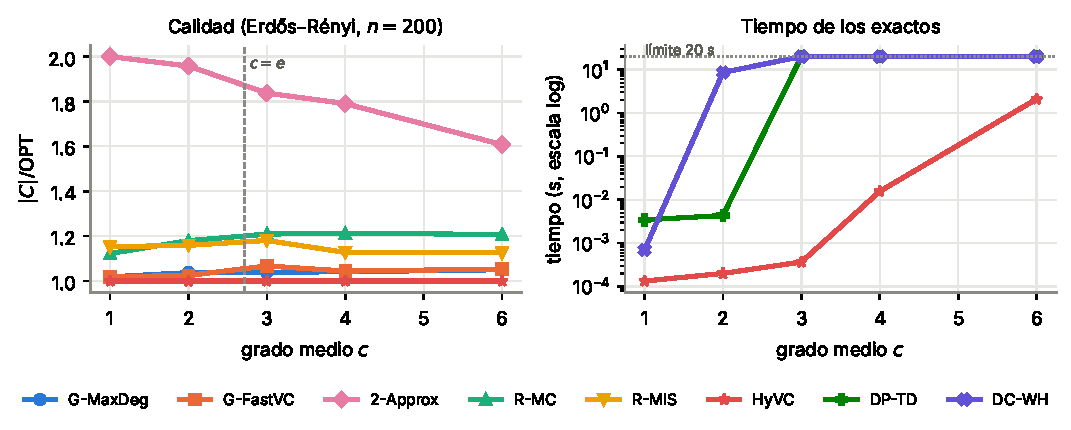
\includegraphics[width=\textwidth]{figs/er_quality_time.pdf}
\caption{Erdős--Rényi con $n=200$. Izquierda: razón media $|C|/\OPT$ de las heurísticas y de \hyvc. Derecha: tiempo medio de los algoritmos exactos; una corrida que no termina cuenta como 20\,s.}
\label{fig:er}
\end{figure}

\subsection{Calidad de las heurísticas}
La \cref{tab:calidad} compara la calidad de las heurísticas con el óptimo. La construcción de FastVC es la mejor heurística en promedio (razón 1.037) y la única que no cae en la trampa de Johnson, donde el greedy de grado máximo llega a $2.95$ veces el óptimo ($k=80$: 288 frente a 80). Fuera de esa familia, el greedy de grado máximo y FastVC quedan entre un 0.5\,\% y un 5\,\% por encima del óptimo. Fuera de la trampa, los dos aleatorizados con garantía de razón $2$ en esperanza (\textsf{R-MC} con $\gamma=1$ y \textsf{R-MIS}) quedan entre un 4\,\% y un 26\,\% por encima, y el matching maximal casi duplica el óptimo, como era de esperar.

\begin{table}[!htbp]\centering\scriptsize\setlength{\tabcolsep}{3.5pt}
\begin{tabular}{@{}lrrrrrr@{}}\toprule
Familia & \textsf{G-MaxDeg} & \textsf{G-FastVC} & \textsf{2-Approx} & \textsf{R-MC} & \textsf{R-MIS} & \textsf{HyVC} \\\midrule
Erdős–Rényi $n{=}200$ & 1.037 & 1.042 & 1.839 & 1.186 & 1.149 & 1.000 \\
Erdős–Rényi $n{=}500$ & 1.050 & 1.046 & 1.864 & 1.242 & 1.144 & 1.000 \\
$k$-árbol parcial $n{=}300$ & 1.005 & 1.023 & 1.891 & 1.221 & 1.149 & 1.000 \\
Banda $n{=}400$ & 1.036$^{4/6}$ & 1.046$^{4/6}$ & 1.416$^{4/6}$ & 1.170$^{4/6}$ & 1.092$^{4/6}$ & 1.000$^{4/6}$ \\
Barabási–Albert $n{=}1000$ & 1.025$^{4/6}$ & 1.046$^{4/6}$ & 1.908$^{4/6}$ & 1.256$^{4/6}$ & 1.185$^{4/6}$ & 1.000$^{4/6}$ \\
Trampa de Johnson & 2.950 & 1.000 & 2.000 & 1.717 & 2.258 & 1.000 \\
Erdős–Rényi denso $n{=}60$ & 1.043 & 1.050 & 1.281 & 1.108 & 1.043 & 1.000 \\
\midrule Todas & 1.168 & 1.037 & 1.790 & 1.237 & 1.218 & 1.000 \\
\bottomrule\end{tabular}
\caption{Razón media $|C|/\OPT$ (1.000 = óptimo). El superíndice $a/b$ indica que el algoritmo solo tiene óptimo certificado en $a$ de las $b$ instancias; la media se calcula sobre esas $a$. Los exactos \textsf{DP-TD} y \textsf{DC-WH} se omiten: cuando terminan su razón es 1 (ver \cref{tab:exactos}).}\label{tab:calidad}\end{table}


En las cuatro instancias que nadie resolvió, la cubierta \emph{anytime} de \hyvc{} queda entre un 3.0\,\% y un 3.9\,\% por encima de la mejor solución de CP-SAT. Nunca es peor que la mejor heurística voraz y es estrictamente mejor en tres de las cuatro (311 frente a 314, 606 frente a 611 y 615 frente a 618). Es un resultado modesto: cuando la búsqueda exacta no termina, \hyvc{} no hace búsqueda local y se queda prácticamente con su cota superior inicial.

\subsection{El parámetro $\gamma$ del greedy aleatorizado}
La \cref{fig:gamma} reproduce el comportamiento que reportan Gao et al.~\citep{gao2018randomized}. Con $\gamma=1$, una sola corrida sobre la trampa de Johnson da $1.99$ veces el óptimo, en línea con la garantía de razón $2$ en esperanza. Al subir $\gamma$ la calidad mejora rápidamente, y con $\gamma\ge 8$ y $16$ corridas se alcanza el óptimo de la trampa (80), donde el greedy determinista obtiene 288. En los grafos aleatorios, repetir 16 veces mejora la razón como mucho en $9$ puntos porcentuales; subir $\gamma$ pesa mucho más que repetir.

\begin{figure}[!htbp]
\centering
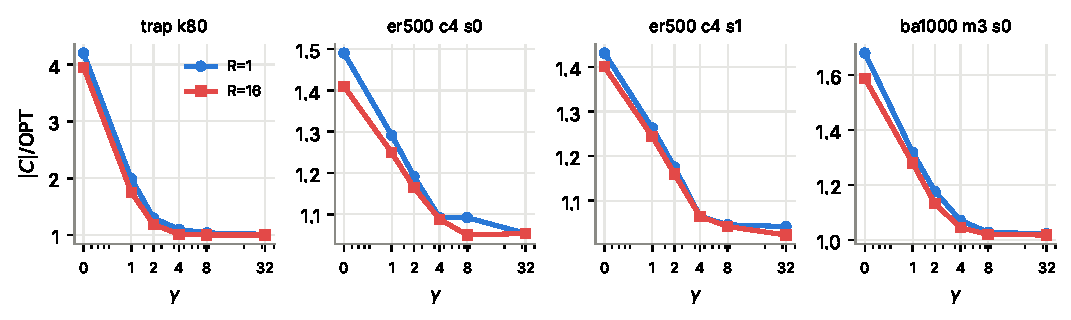
\includegraphics[width=\textwidth]{figs/gamma.pdf}
\caption{Greedy aleatorizado $\deg^\gamma$: razón $|C|/\OPT$ en función de $\gamma$, con una corrida ($R=1$) y con la mejor de 16 ($R=16$).}
\label{fig:gamma}
\end{figure}

\subsection{Qué sección hace el trabajo: ablación}
La \cref{tab:hyvc} muestra dónde trabaja \hyvc{} en cada familia, y la \cref{tab:ablacion} y la \cref{fig:ablacion} apagan una sección a la vez, con un límite de 10\,s.

\begin{table}[!htbp]\centering\small
\begin{tabular}{@{}lrrrr@{}}\toprule
Familia & núcleo tras reducir & comp.\ a PD & comp.\ a B\&R & nodos B\&R (media) \\\midrule
Erdős–Rényi $n{=}200$ & 23.0\% & 0 & 5 & 538 \\
Erdős–Rényi $n{=}500$ & 23.3\% & 0 & 2 & 391 \\
$k$-árbol parcial $n{=}300$ & 0.0\% & 0 & 0 & 0 \\
Banda $n{=}400$ & 93.7\% & 4 & 3 & 59 \\
Barabási–Albert $n{=}1000$ & 33.3\% & 0 & 2 & 4771 \\
Trampa de Johnson & 0.0\% & 0 & 0 & 0 \\
Erdős–Rényi denso $n{=}60$ & 100.0\% & 0 & 3 & 150 \\
\bottomrule\end{tabular}
\caption{Qué sección de \hyvc{} hace el trabajo: fracción de vértices que sobrevive a las reducciones, componentes despachadas a programación dinámica o a branch \& reduce, y nodos de búsqueda.}\label{tab:hyvc}\end{table}


\begin{itemize}
  \item \textbf{Reducciones} (Ásgeirsson--Stein, Akiba--Iwata). Es la sección más importante. Resuelve por completo los $k$-árboles parciales y la trampa de Johnson, deja núcleos del 23\,\% en los Erdős--Rényi y del 33\,\% en los Barabási--Albert, y sin ella \hyvc{} pasa de 10/10 a 6/10 instancias exactas en Erdős--Rényi y de 4/6 a 0/6 en Barabási--Albert.
  \item \textbf{Programación dinámica} (Bannach--Berndt, Alber et al.). Es decisiva en las bandas: sin ella, \hyvc{} pasa de 4/6 a 1/6 instancias exactas y de 37 a más de 27\,000 nodos de búsqueda en promedio. En los Erdős--Rényi tiene un costo neto: estimar $\kappa(H)$ en cada nodo hace que \hyvc{} completo tarde 0.37\,s frente a 0.21\,s sin PD.
  \item \textbf{División en componentes} (Weigt--Hartmann) y \textbf{cota Monte Carlo} (Gao et al.). En estas instancias no tienen un efecto medible: apagarlas no cambia ni el número de instancias exactas ni el tiempo más allá del ruido. Después de las reducciones, los núcleos son casi siempre una sola componente grande que la búsqueda no alcanza a fragmentar en 10\,s, y la cota superior voraz ya está a pocos vértices del óptimo, así que la búsqueda pasa casi todo su tiempo probando la cota inferior y no mejorando la superior.
\end{itemize}

\begin{table}[!htbp]\centering\small
\begin{tabular}{@{}llrrr@{}}\toprule
Familia & Variante & $\bar t$ (s) & exactas & nodos \\\midrule
Erdős–Rényi $n{=}200$ & HyVC completo & 0.37 & 10/10 & 481 \\
 & sin reducciones & 5.38 & 6/10 & 44 \\
 & sin DP & 0.21 & 10/10 & 561 \\
 & sin division & 0.40 & 10/10 & 484 \\
 & sin Monte Carlo & 0.37 & 10/10 & 486 \\
\addlinespace
Banda $n{=}400$ & HyVC completo & 3.72 & 4/6 & 37 \\
 & sin reducciones & 3.82 & 4/6 & 40 \\
 & sin DP & 8.50 & 1/6 & 27573 \\
 & sin division & 3.73 & 4/6 & 34 \\
 & sin Monte Carlo & 3.74 & 4/6 & 39 \\
\addlinespace
Barabási–Albert $n{=}1000$ & HyVC completo & 3.36 & 4/6 & 2572 \\
 & sin reducciones & 10.26 & 0/6 & 238 \\
 & sin DP & 3.36 & 4/6 & 3840 \\
 & sin division & 3.36 & 4/6 & 2351 \\
 & sin Monte Carlo & 3.35 & 4/6 & 2307 \\
\bottomrule\end{tabular}
\caption{Ablación: se apaga una sección de \hyvc{} a la vez (límite 10\,s). Si una variante no termina, aporta 10\,s a la media.}\label{tab:ablacion}\end{table}


\begin{figure}[!htbp]
\centering
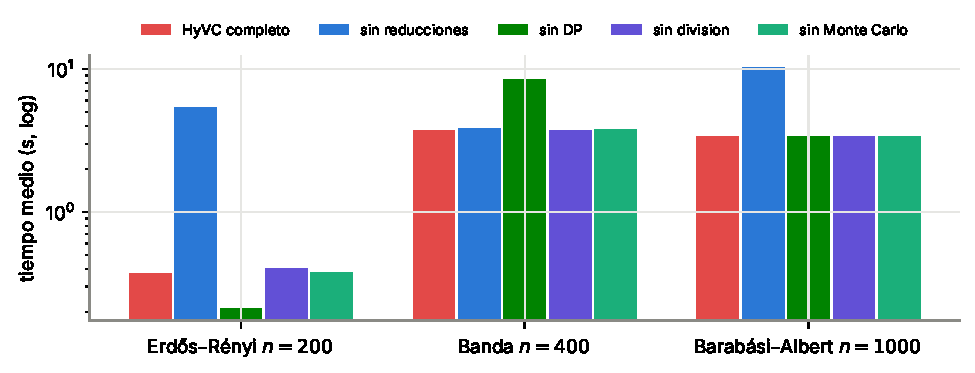
\includegraphics[width=0.85\textwidth]{figs/ablation.pdf}
\caption{Ablación: tiempo medio de \hyvc{} al apagar una sección (escala logarítmica, límite 10\,s).}
\label{fig:ablacion}
\end{figure}

\subsection{Amenazas a la validez}
Todas las implementaciones, \hyvc{} incluido, están en Python. Los tiempos absolutos no son comparables con implementaciones en C++ como las de los artículos originales; solo lo son las comparaciones relativas dentro de este trabajo. Las instancias son sintéticas y de tamaño moderado (hasta 1000 vértices). Usamos 2 o 3 semillas por configuración, así que las diferencias pequeñas de tiempo no son significativas. El ancho de árbol se estima con una sola heurística (grado mínimo); una mejor descomposición ampliaría el régimen de la PD. Por último, los parámetros de \hyvc{} ($\kappa_{\max}$, el tope interno, $\gamma$ y $R$) se fijaron a mano, y la elección de $\gamma=2$ es subóptima según la \cref{fig:gamma}.


\section{Conclusiones}\label{sec:conclusiones}
Comparamos sección por sección cinco algoritmos publicados para \textsc{Minimum Vertex Cover}, uno o dos por paradigma (voraz, programación dinámica, divide y vencerás y aleatorizado), y con esa comparación construimos \hyvc. El híbrido reduce el grafo con reglas exactas, lo divide en componentes, despacha a programación dinámica las componentes cuya tabla es barata y ramifica sobre el resto con poda por cotas. Siempre devuelve una cubierta válida y, si termina, óptima.

En 46 instancias de seis familias, \hyvc{} certificó el óptimo en 42, frente a 20 del divide y vencerás de Weigt y Hartmann y 17 de la programación dinámica sobre descomposiciones en árbol. Los dos algoritmos base solo funcionan en su régimen; \hyvc{} cubre la unión de ambos y además resuelve familias que ninguno cierra. La ablación muestra que la ganancia no se reparte por igual: casi todo el efecto viene de las reglas de reducción y, en grafos de ancho de árbol pequeño, de la programación dinámica. La división dinámica en componentes y la cota superior Monte Carlo, que en la comparación teórica parecían prometedoras, no tuvieron un efecto medible en estas instancias.

El desarrollo también dejó una lección de diseño: el criterio para despachar a programación dinámica debe ser un \emph{costo} estimado, y no un umbral de ancho. Con un umbral fijo, \hyvc{} no despachaba grafos que la PD resolvía en centésimas de segundo; con un único tope de costo, gastaba segundos en tablas que la ramificación resolvía en milisegundos.

\paragraph{Trabajo futuro.} (i) Añadir una fase de búsqueda local (por ejemplo, la de FastVC o NuMVC) para que la respuesta \emph{anytime} mejore cuando la búsqueda exacta no termina; (ii) cotas inferiores más fuertes, como la relajación LP o una cobertura por cliques~\citep{akiba2016branch}, para cerrar las instancias densas y de ley de potencias; (iii) reemplazar la descomposición por grado mínimo por una mejor (p.\,ej. la heurística de \emph{min-fill} o un solucionador de treewidth); (iv) ajustar $\gamma$ automáticamente, ya que valores $\gamma\ge 8$ resultaron claramente mejores que el $\gamma=2$ usado; y (v) explorar la ramificación aleatorizada de Clinch et al.~\citep{clinch2025faster} como alternativa Las Vegas a la ramificación determinista.


\bibliographystyle{plainnat}
\bibliography{refs}

\appendix
\section{Código}\label{app:codigo}
El código está organizado como sigue (ejecutar desde la raíz del proyecto):
\begin{itemize}
  \item \texttt{vc/greedy.py}, \texttt{vc/randomized.py}, \texttt{vc/dp\_treedec.py}, \texttt{vc/divide\_conquer.py}: algoritmos base.
  \item \texttt{vc/reductions.py} y \texttt{vc/hybrid.py}: reglas R0--R4 y \hyvc.
  \item \texttt{tests/}: pruebas contra fuerza bruta y contra CP-SAT.
  \item \texttt{bench/run\_experiments.py} y \texttt{bench/make\_figures.py}: experimentos, tablas y figuras de este documento.
\end{itemize}

\end{document}
